\documentclass[10pt,a4paper,twocolumn]{article}

\usepackage[utf8]{inputenc}
\usepackage[T1]{fontenc}
\usepackage{mathptmx}
\usepackage[a4paper,top=2.0cm,bottom=2.1cm,left=1.9cm,right=1.9cm,columnsep=0.7cm]{geometry}
\usepackage{amsmath,amssymb}
\usepackage{array,tabularx}
\usepackage{graphicx}
\usepackage{float}
\usepackage[table]{xcolor}
\usepackage{caption}
\usepackage{listings}
\usepackage{tikz}
\usetikzlibrary{arrows.meta,positioning,calc,fit}
\usepackage{titlesec}
\usepackage{fancyhdr}
\PassOptionsToPackage{hyphens}{url}
\usepackage[hidelinks]{hyperref}
\urlstyle{same}
\sloppy
\setlength{\parindent}{1.2em}
\setlength{\parskip}{0pt}
\linespread{1.02}

\titleformat{\section}{\large\bfseries}{\thesection}{0.6em}{}
\titleformat{\subsection}{\normalsize\bfseries}{\thesubsection}{0.6em}{}
\titleformat{\subsubsection}{\normalsize\bfseries}{}{0em}{}
\titlespacing*{\section}{0pt}{11pt plus 2pt}{5pt}
\titlespacing*{\subsection}{0pt}{8pt plus 2pt}{3pt}
\titlespacing*{\subsubsection}{0pt}{6pt plus 2pt}{2pt}

\captionsetup{font=small,labelfont=bf,labelsep=period,justification=justified,singlelinecheck=off}
\captionsetup[table]{position=above,skip=4pt}
\captionsetup[figure]{position=below,skip=4pt}
\renewcommand{\lstlistingname}{Listing}
\captionsetup[lstlisting]{position=above}

\lstset{
  basicstyle=\ttfamily\scriptsize,
  breaklines=true,
  frame=single,
  framerule=0.3pt,
  columns=fullflexible,
  keepspaces=true,
  showstringspaces=false,
  captionpos=t,
  aboveskip=6pt,belowskip=6pt
}

\pagestyle{fancy}
\fancyhf{}
\fancyhead[C]{\small Lane Detection System}
\fancyfoot[C]{\small\thepage}
\renewcommand{\headrulewidth}{0pt}
\fancypagestyle{firstpage}{\fancyhf{}\fancyfoot[C]{\small\thepage}\renewcommand{\headrulewidth}{0pt}}

\renewcommand{\arraystretch}{1.12}
\setlength{\tabcolsep}{3.5pt}

\begin{document}

\twocolumn[{%
\begin{center}
{\LARGE\bfseries Lane Detection System Combining Traditional Computer Vision\\[2pt] with Pixel-Wise Machine Learning\par}
\vspace{9pt}
{\large Sujal, Nitish Gupta\par}
\vspace{3pt}
{\small\itshape Department of Electronics and Communication Engineering, Bharati Vidyapeeth College of Engineering, Pune, India\par}
\end{center}
\vspace{2pt}
\noindent{\large\bfseries Abstract}\par\vspace{3pt}
\noindent\small
Lane detection is a core perception task for driver assistance and autonomous driving. Classical image-processing methods identify lane-like edges efficiently, but their output is sensitive to illumination, shadows, worn markings, and road texture. This report specifies a hybrid lane-detection system in which traditional computer vision narrows the region and constructs visual cues, while a convolutional neural network predicts lane pixels from image context. The design uses a trapezoidal road region of interest (ROI), color and grayscale conversion, Gaussian smoothing, Canny edge detection, morphological filtering, and optional Hough line segments. A U-Net-style encoder--decoder is proposed to classify each road pixel as lane marking or background. The report defines a reproducible training and evaluation plan using the CULane benchmark, sequence-aware data splits, aligned masks and augmentation, weighted binary cross-entropy plus Dice loss, and pixel accuracy, precision, recall, Dice/F1, and intersection over union (IoU). No dataset, trained weights, or measured predictions were supplied; therefore no empirical scores are claimed. Dashboard images document the prototype interface only. The result is a project specification for implementation and controlled comparison of hybrid inputs against a CNN-only baseline.

\vspace{5pt}
\noindent\textbf{Keywords:} lane detection, computer vision, semantic segmentation, U-Net, Canny edge detection, Hough transform, IoU, driver assistance
\vspace{8pt}
}]
\thispagestyle{firstpage}
\begingroup\renewcommand{\thefootnote}{}%
\footnotetext{\footnotesize Code repositories: \url{https://github.com/Sujal-48/Lane-Detection-System} | \url{https://github.com/nitishgupta2764-cmd/Lane-Detection-System}}%
\endgroup

\section{Introduction}
A lane-detection system estimates the position and shape of painted lane boundaries in a forward-facing road image. The estimate can support lane-departure warning, lane-keeping assistance, road-scene understanding, and mapping. Markings may be faint, occluded, curved, or visually similar to road repairs and shadows; camera motion, perspective, weather, and exposure further alter their appearance.

Traditional vision offers interpretable, economical operations: an ROI suppresses irrelevant areas, color thresholds distinguish some paint colors, edge detectors emphasize intensity transitions, and the Hough transform identifies approximately straight segments. Fixed thresholds and geometric assumptions can fail on worn, curved, or obscured markings. A learned pixel classifier can use broader context but requires labeled data and compute and remains vulnerable to domain shift.

This project combines the approaches in a staged system. Classical processing produces a constrained candidate map and auxiliary channels; a segmentation network predicts lane pixels from the image plus those cues. Edge and Hough maps are inputs or post-processing aids, not substitutes for the learned decision. The objectives are to build the preprocessing pipeline, train a pixel-wise classifier, compare hybrid inputs against a CNN-only baseline, evaluate segmentation and runtime, and document a reproducible ECE project path.

\subsection{Objectives and Contributions}
The work is organized around five concrete objectives.
\textbf{(O1)} Implement a deterministic classical front end that converts a road frame into an ROI mask and edge cues.
\textbf{(O2)} Train a compact U-Net-style segmenter that predicts a per-pixel lane probability.
\textbf{(O3)} Run a controlled ablation that compares RGB, RGB+ROI, RGB+edge, and RGB+ROI+edge inputs under identical data, capacity, and training budget.
\textbf{(O4)} Evaluate overlap quality and runtime with a protocol fixed before test data are examined.
\textbf{(O5)} Package code, configuration, split manifest, and logs so that another student can repeat the study.

The contribution of this report is a specification rather than a measured result: it fixes the interfaces, the data handling rules, the loss, the metrics, and the reporting templates, so that the eventual experiment can be judged against criteria written down in advance. This ordering protects against the common failure mode in small projects, where thresholds and checkpoints are tuned on the same frames that are later reported.

\subsection{Organization of the Report}
Section~\ref{sec:background} reviews classical and learned lane detection. Section~\ref{sec:problem} states the problem, requirements, and scope. Section~\ref{sec:arch} describes the architecture and module interfaces. Sections~\ref{sec:data} to~\ref{sec:model} detail the dataset, the traditional vision stage, and the pixel-wise model. Section~\ref{sec:eval} defines evaluation, Section~\ref{sec:results} gives the results template and dashboard demonstration, Sections~\ref{sec:discussion} and~\ref{sec:limits} discuss interpretation and limitations, and Section~\ref{sec:repro} lists reproducibility artifacts, a work plan, and future directions.

\section{Background and Related Work}\label{sec:background}
Classical lane pipelines apply color or gradient thresholds inside a road ROI and fit line or curve models. Canny edge detection uses smoothing, gradient estimation, non-maximum suppression, and hysteresis thresholding \cite{canny1986}. The Hough transform identifies lines supported by multiple edge points. These methods provide useful candidate evidence, especially on near-straight highways, but road boundaries, vehicle edges, seams, and shadows create competing responses.

Semantic segmentation predicts a class for each pixel. U-Net combines contextual features from a contracting path with high-resolution features from a decoder through skip connections \cite{ronneberger2015}. LaneNet frames lane detection as lane-edge proposal and localization \cite{neven2018a}. This project adopts a compact U-Net-style binary segmenter as a project-scale baseline. Its central hypothesis is that ROI and edge cues may improve the model under identical data and compute conditions; this is to be tested, not assumed.

\subsection{Classical Lane Pipelines}
A typical classical pipeline has four steps: restrict the image to a road region, enhance paint contrast through color or gradient operations, extract candidate boundary pixels, and fit a geometric model. Straight-line models are cheap and work well on highways with small curvature; polynomial or spline models extend the approach to bends. The weakness is brittleness. Each step carries parameters that depend on camera height, field of view, resolution, and lighting, and an error early in the chain propagates unchecked to the final fit. For this reason the present design saves every intermediate image and keeps the geometric fit separate from classification scores.

\subsection{Learning-Based Lane Detection}
Learning-based methods replace hand-set thresholds with parameters estimated from labeled frames. Spatial CNN (SCNN) passes information across rows and columns inside a feature map to model thin, long structures such as lanes, and introduced the CULane benchmark \cite{pan2018}. LaneNet separates lane-edge proposal from instance embedding so that individual lanes can be told apart \cite{neven2018a,neven2018b}. Segmentation-style networks are attractive for a student project because the training signal is dense, the code is short, and the output is directly viewable as an overlay. Their costs are labeled data, GPU time, and sensitivity to a mismatch between training and deployment cameras.

\subsection{Hybrid Approaches and the Gap Addressed}
Hybrid designs feed hand-crafted evidence to a network, or use classical geometry to clean up network output. The open question for a small system is whether such evidence adds anything once the network sees the raw image, since a convolutional encoder can in principle learn edge filters itself. The ablation in Section~\ref{sec:ablation} isolates that question by changing only the input channels, so any measured difference can be attributed to the cues and not to a different model or training budget.

\begin{table}[H]
\centering
\caption{Candidate datasets and their intended roles. Counts are to be copied from the official releases.}
\footnotesize
\begin{tabularx}{\columnwidth}{|l|X|X|}
\hline
\rowcolor{gray!18}\textbf{Dataset}&\textbf{Role in this project}&\textbf{Notes to verify}\\ \hline
CULane & Primary training, validation, and test source & Urban scenes; nine scenario categories; check release and terms\\ \hline
TuSimple & Optional cross-dataset check & Highway-style scenes; check documentation and license\\ \hline
BDD100K & Optional diversity check & Multitask driving dataset; use lane labels only if terms permit\\ \hline
\end{tabularx}
\end{table}

\section{Problem Statement and Scope}\label{sec:problem}
Given a forward-facing RGB image $I$ of height $H$ and width $W$, estimate a binary mask $M\in\{0,1\}^{H\times W}$, where 1 denotes a visible lane marking. The system should suppress predictions outside a plausible road region, preserve thin markings, and produce an inspectable overlay. The initial scope is single-frame, 2D camera-based segmentation; it does not estimate metric road geometry, vehicle pose, or steering commands. Lane-instance classes are optional when labels support them. The prototype is academic and is not safety-certified.

\subsection{Formal Statement}
Let $I\in[0,1]^{3\times H\times W}$ be the normalized image and $R\in\{0,1\}^{H\times W}$ the ROI mask. The classical front end is a deterministic function $C$ that returns a cue tensor, and the network $f_\theta$ returns one logit per pixel. The predicted mask is the thresholded probability restricted to the ROI:
\begin{align}
x &= [\,I\,;\,C(I)\,], \qquad p = \sigma\big(f_\theta(x)\big), \\
M_{\mathrm{pred}} &= \mathbf{1}[\,p\ge\tau\,]\odot R,
\end{align}
where $\sigma$ is the logistic function, $\tau$ is the validation-selected threshold, and the product is taken element by element. The parameters $\theta$ are estimated on training sequences only; $\tau$ and the ROI are chosen on validation sequences only.

\subsection{Requirements}
\begin{table}[H]
\centering
\caption{Functional and process requirements.}
\footnotesize
\begin{tabularx}{\columnwidth}{|l|X|X|}
\hline
\rowcolor{gray!18}\textbf{ID}&\textbf{Requirement}&\textbf{Check}\\ \hline
R1 & Accept an RGB frame and validate its size & Unit test on bad input\\ \hline
R2 & Produce identical cues at training and inference & Hash of cue tensors on fixed frames\\ \hline
R3 & Output a probability map, a mask, and an overlay & Visual review on fixed IDs\\ \hline
R4 & Never use test labels for any tuning step & Test split read-only until freeze\\ \hline
R5 & Report overlap metrics and latency separately & Evaluation script output\\ \hline
R6 & Log seed, versions, and configuration with every run & Run folder inspection\\ \hline
\end{tabularx}
\end{table}

\subsection{Out of Scope}
Metric road geometry, ego-vehicle pose, steering or braking decisions, multi-camera fusion, and temporal tracking are outside this project. Real-time operation on embedded hardware is a stated future direction and is not claimed here.

\section{System Architecture}\label{sec:arch}
Training converts frames and annotations into aligned tensors, generates deterministic classical cues, and trains the segmenter on image-plus-cue inputs. Inference applies the same preprocessing, predicts a probability map, and uses a validation-selected threshold and optional geometric filtering.

The hybrid baseline input is RGB plus ROI and Canny/morphology channels. Ablations compare RGB, RGB+ROI, RGB+edge, and RGB+ROI+edge; optional Hough features are included only if deterministic and independent of test labels.

\begin{figure}[H]
\centering
\resizebox{\columnwidth}{!}{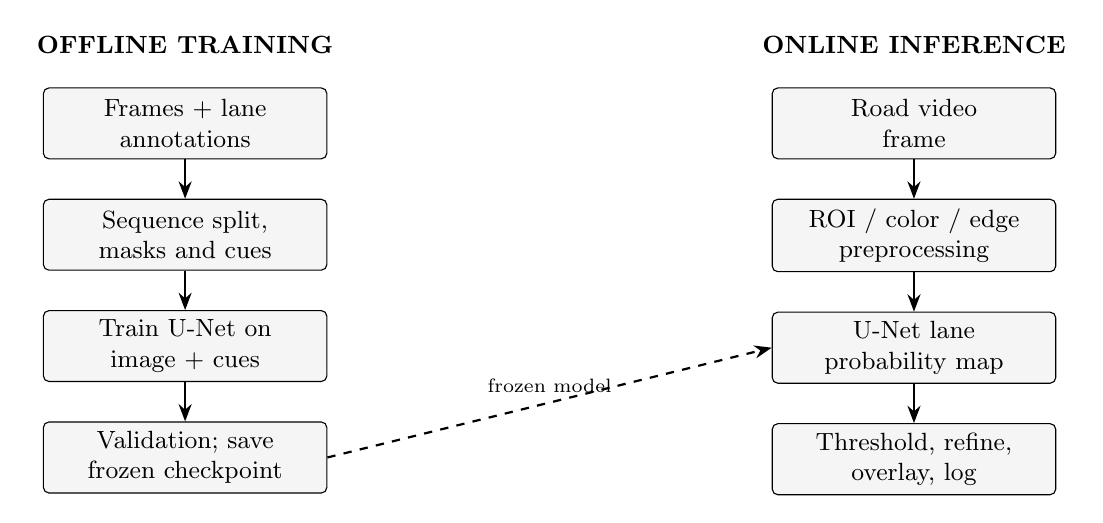
\begin{tikzpicture}[
  node distance=5mm,
  box/.style={draw,rounded corners=2pt,align=center,minimum width=3.6cm,minimum height=0.9cm,font=\small,fill=gray!8},
  arr/.style={-{Stealth[length=2.2mm]},thick}]
\node[font=\small\bfseries] (t1) {OFFLINE TRAINING};
\node[box,below=3mm of t1] (a1) {Frames + lane\\annotations};
\node[box,below=of a1] (a2) {Sequence split,\\masks and cues};
\node[box,below=of a2] (a3) {Train U-Net on\\image + cues};
\node[box,below=of a3] (a4) {Validation; save\\frozen checkpoint};
\node[font=\small\bfseries,right=5.2cm of t1] (t2) {ONLINE INFERENCE};
\node[box,below=3mm of t2] (b1) {Road video\\frame};
\node[box,below=of b1] (b2) {ROI / color / edge\\preprocessing};
\node[box,below=of b2] (b3) {U-Net lane\\probability map};
\node[box,below=of b3] (b4) {Threshold, refine,\\overlay, log};
\foreach \u/\v in {a1/a2,a2/a3,a3/a4,b1/b2,b2/b3,b3/b4} \draw[arr] (\u) -- (\v);
\draw[arr,dashed] (a4.east) -- node[above,font=\scriptsize]{frozen model} (b3.west);
\end{tikzpicture}}
\caption{System architecture. Training produces a frozen model; inference applies the same deterministic cues before pixel-wise prediction and optional refinement.}
\end{figure}

\subsection{Module Decomposition}
\begin{table}[H]
\centering
\caption{Modules and interfaces.}
\footnotesize
\begin{tabularx}{\columnwidth}{|l|X|X|}
\hline
\rowcolor{gray!18}\textbf{Module}&\textbf{Input}&\textbf{Output}\\ \hline
Loader & Video or image path & RGB array, frame ID\\ \hline
ROI & Image shape, ROI config & Binary road mask $R$\\ \hline
Edge cue & Grayscale frame & Binary edge map $E$\\ \hline
Assembler & RGB, $R$, $E$ & Normalized tensor $x$\\ \hline
Segmenter & Tensor $x$ & Probability map $p$\\ \hline
Refiner & $p$, $\tau$, $R$ & Mask $M_{\mathrm{pred}}$, overlay\\ \hline
Logger & Frame ID, $p$, latency & Per-frame log record\\ \hline
\end{tabularx}
\end{table}

\subsection{Input Channel Layout}
The network input is a stack of channels in a fixed order so that checkpoints and cue generators cannot be mismatched. Channels 0 to 2 are R, G, B in that order after explicit color-order conversion from the decoder's native order. Channel 3 is the binary ROI mask and channel 4 is the binary edge map after morphology. An optional channel 5 holds Hough-segment support. Binary channels are not mean-subtracted; they stay in $\{0,1\}$ so that they remain interpretable.

\begin{figure}[H]
\centering
\resizebox{\columnwidth}{!}{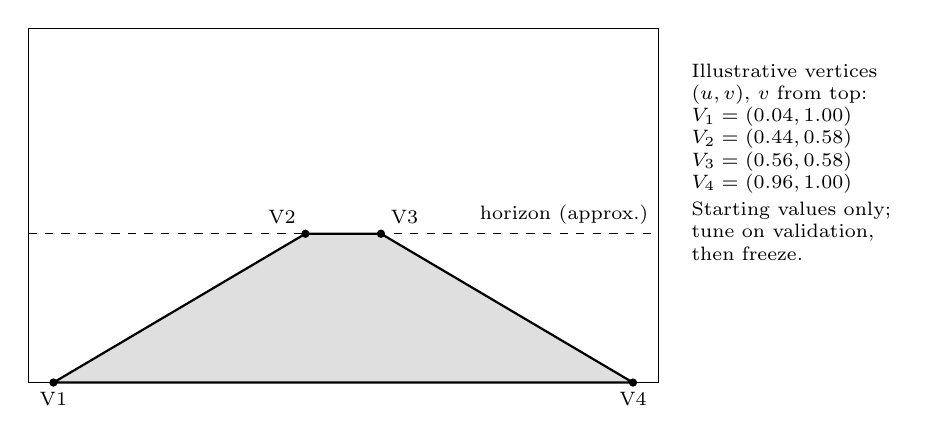
\begin{tikzpicture}[scale=1]
\draw (0,0) rectangle (8,4.5);
\coordinate (V1) at (0.32,0);
\coordinate (V2) at (3.52,1.89);
\coordinate (V3) at (4.48,1.89);
\coordinate (V4) at (7.68,0);
\fill[gray!25] (V1) -- (V2) -- (V3) -- (V4) -- cycle;
\draw[thick] (V1) -- (V2) -- (V3) -- (V4) -- cycle;
\draw[dashed] (0,1.89) -- (8,1.89) node[above left,font=\scriptsize]{horizon (approx.)};
\foreach \p/\l/\a in {V1/V1/below,V2/V2/above left,V3/V3/above right,V4/V4/below}
  {\fill (\p) circle (1.5pt); \node[font=\scriptsize,\a] at (\p) {\l};}
\node[font=\scriptsize,align=left,anchor=west] at (8.3,2.8) {Illustrative vertices\\$(u,v)$, $v$ from top:\\
$V_1=(0.04,1.00)$\\$V_2=(0.44,0.58)$\\$V_3=(0.56,0.58)$\\$V_4=(0.96,1.00)$\\[2pt]
Starting values only;\\tune on validation,\\then freeze.};
\end{tikzpicture}}
\caption{Trapezoidal ROI in normalized coordinates, wide at the near road and narrow near the horizon. Vertices are illustrative starting values, not tuned results.}
\end{figure}

\subsection{Configuration as a Single Source of Truth}
Every parameter that influences a tensor, a threshold, or a metric lives in one machine-readable configuration file saved with the checkpoint. The inference code reads the same file. This removes the common error in which a model is trained with one ROI or Canny setting and deployed with another.

\subsection{Per-Frame Log Record}
Each processed frame writes one machine-readable record so that failures can be traced after the run. The record is deliberately small, and it never stores the frame itself, which keeps logs shareable even when dataset terms forbid redistributing images.

\begin{table}[H]
\centering
\caption{Per-frame log fields.}
\footnotesize
\begin{tabularx}{\columnwidth}{|l|X|}
\hline
\rowcolor{gray!18}\textbf{Field}&\textbf{Content}\\ \hline
\texttt{frame\_id} & Sequence name and frame index\\ \hline
\texttt{t\_pre, t\_net, t\_post} & Stage times in milliseconds\\ \hline
\texttt{mean\_prob} & Mean of $p$ inside the ROI\\ \hline
\texttt{lane\_pixels} & Count of mask pixels after refinement\\ \hline
\texttt{components} & Connected components kept / removed\\ \hline
\texttt{config\_hash} & Hash of the frozen configuration\\ \hline
\end{tabularx}
\end{table}

\subsubsection*{Frame-by-Frame Inference Pseudocode}
Load the validation-selected checkpoint and preprocessing configuration once, then apply the same deterministic operations to every decoded frame. The network predicts lane probabilities; the ROI and optional component filter only constrain and refine that output.

\begin{lstlisting}
function process_video(video, checkpoint):
  model, config, tau = load_checkpoint(checkpoint)
  stats = config.training_normalization
  for frame_id, frame in decode_frames(video):
    start = clock()
    rgb = decode_as_RGB(frame)
    roi = trapezoid_mask(rgb.shape, config.roi)
    gray = convert_to_grayscale(rgb)
    smooth = gaussian_blur(gray, kernel=5x5)
    edge = canny(smooth, config.frozen_canny_thresholds)
    edge = morphology(edge, config.morphology)
    cues = concatenate(roi, edge)
    x = normalize(concatenate(rgb, cues), stats)
    probability = sigmoid(model(x))
    mask = (probability >= tau) AND roi
    mask = remove_tiny_components(mask, config.min_size)
    overlay = draw_mask(rgb, mask)
    latency = clock() - start
    display_or_save(frame_id, overlay)
    log(frame_id, mean(probability), latency)
  return saved_overlays, frame_log
\end{lstlisting}

\begin{table}[H]
\centering
\caption{Processing stages and outputs.}
\footnotesize
\begin{tabularx}{\columnwidth}{|l|X|}
\hline
\rowcolor{gray!18}\textbf{Stage}&\textbf{Operation and output}\\ \hline
Input & Read RGB frame and validate dimensions\\ \hline
Traditional vision & ROI, grayscale/color transforms, blur, Canny and morphology cues\\ \hline
Feature assembly & Normalize and concatenate image and selected cues\\ \hline
Pixel classifier & U-Net encoder--decoder produces a lane probability map\\ \hline
Refinement & Threshold, restrict to ROI, optionally remove tiny components or fit curves\\ \hline
Presentation & Overlay mask and save diagnostics\\ \hline
\end{tabularx}
\end{table}

\section{Dataset and Preprocessing}\label{sec:data}
CULane is the recommended primary dataset because it covers varied urban driving conditions, including night, shadow, crowd, and curve cases \cite{pan2018}. Record its exact version, terms, and split manifest. Lane geometry must be rasterized into masks using one documented line width at the chosen resolution. Keep annotation gaps or out-of-view points consistent with dataset conventions; do not interpolate across large missing regions. A documented subset may be used when resources are limited.

Split by video sequence where metadata permit to avoid leakage between near-identical neighboring frames. Decode consistently into RGB. Resize image and mask to a fixed input such as $512\times288$ or $640\times360$; use bilinear interpolation for images and nearest-neighbor for categorical masks. Apply geometric transforms jointly to image and mask, while photometric augmentation affects only the image. Normalize to $[0,1]$ or use channel statistics computed from training data only. Freeze ROI vertices, thresholds, mask width, and probability threshold before test evaluation.

Define a trapezoidal ROI in normalized coordinates, wide at the near road and narrower near the horizon. Use grayscale for gradients and optional HSV or Lab channels for color cues. Treat color thresholds as candidates because paint, white balance, and illumination vary. Preserve the exact split IDs and preprocessing configuration with the model.

Before implementation, obtain CULane from its official distribution and record the release, license or terms that apply, and the exact train, validation, and test manifest. If storage or compute requires a subset, select it by sequence, state exact counts, and keep a fixed manifest for every ablation. CULane annotations are commonly lane geometry rather than ready-made thick binary masks. Connect consecutive visible points and rasterize a narrow line at the chosen training resolution. Choose the width once and record it in configuration. Leave out-of-view points and annotation gaps as background or ignored pixels according to the dataset convention; never bridge a large missing interval by interpolation. Inspect overlays from all scene types before training.

If aspect ratio is preserved, document the padding or crop used to reach the network tensor size. Geometric operations such as horizontal flips, crops, translations, and warps must be applied jointly to image and mask. Use nearest-neighbor interpolation for categorical masks so resize does not introduce fractional classes. Photometric brightness or contrast changes affect only the image. Compute normalization statistics from training frames only. Tune ROI coordinates, edge thresholds, mask width, probability threshold, and checkpoint selection using validation data only; keep test data read-only until the design is frozen.

\subsection{Scenario Categories}
CULane test frames are tagged with scenario categories. Reporting per category exposes failures that a single global score hides, so the category tags are carried through the manifest.

\begin{table}[H]
\centering
\caption{Scenario categories used for condition-wise reporting. Exact counts are to be taken from the manifest.}
\footnotesize
\begin{tabularx}{\columnwidth}{|l|X|}
\hline
\rowcolor{gray!18}\textbf{Category}&\textbf{Why it matters for this design}\\ \hline
Normal & Reference condition; sanity check\\ \hline
Crowded & Vehicle edges compete with paint edges\\ \hline
Dazzle light & Saturation hides gradients\\ \hline
Shadow & Strong false edges across the road\\ \hline
No line & Faint or absent paint; tests recall and false positives\\ \hline
Arrow & Road symbols resemble short lane segments\\ \hline
Curve & Stresses a fixed trapezoidal ROI\\ \hline
Crossroad & Many non-lane markings and missing lanes\\ \hline
Night & Low contrast, headlight glare\\ \hline
\end{tabularx}
\end{table}

\subsection{Mask Rasterization Procedure}
Because annotations are polylines, the mask depends on a few choices that are easy to forget: the line width, the anti-aliasing setting, and the order of resize and rasterization. The procedure below rasterizes at the training resolution directly from rescaled coordinates, which avoids resampling a thin line and then thresholding it.

\begin{lstlisting}[caption={Lane polyline rasterization.}]
function rasterize_lanes(points, width, ignore_policy):
  mask = zeros(H_train, W_train)
  for lane in points:
    pts = rescale(lane, src_size, (W_train, H_train))
    for a, b in consecutive_visible_pairs(pts):
      if gap_length(a, b) > ignore_policy.max_gap:
        continue   # never bridge a large gap
      draw_line(mask, a, b, value=1, thickness=width,
                antialias=False)
  return mask
\end{lstlisting}

\subsection{Sequence-Level Splitting}
Neighboring video frames are nearly identical. If they fall on both sides of a split, validation and test scores measure memorization of a scene and not generalization. The manifest therefore groups frames by recording sequence and assigns whole groups to one split. When the official CULane lists already separate sequences, those lists are used unchanged and only a validation subset is carved from the training sequences, again by sequence.

\subsection{Augmentation Policy}
\begin{table}[H]
\centering
\caption{Augmentation policy. A library such as Albumentations \cite{buslaev2020} can apply image and mask transforms jointly.}
\footnotesize
\begin{tabularx}{\columnwidth}{|l|l|X|}
\hline
\rowcolor{gray!18}\textbf{Operation}&\textbf{Applies to}&\textbf{Note}\\ \hline
Brightness / contrast jitter & Image only & Moderate range\\ \hline
Small translation / scale & Image, mask, cues & Joint transform\\ \hline
Mild Gaussian blur & Image only & Cues recomputed after\\ \hline
Horizontal flip & Image, mask, cues & Only if convention holds\\ \hline
Vertical flip & Not used & Physically implausible\\ \hline
\end{tabularx}
\end{table}

An important detail concerns cues. If a geometric transform moves the image, the ROI and edge channels must follow it. The simplest safe rule is to augment the RGB frame and mask first and then recompute the edge cue from the augmented frame, so that cue and image can never disagree.

\subsection{Data Inspection Before Training}
Visual inspection is the cheapest defense against silent label errors. Before the first training run, render a fixed random sample of frames from every scenario category with the rasterized mask and the ROI drawn over the image, and review them at native resolution.

\begin{table}[H]
\centering
\caption{Pre-training inspection checklist.}
\footnotesize
\begin{tabularx}{\columnwidth}{|l|X|}
\hline
\rowcolor{gray!18}\textbf{Check}&\textbf{What a failure looks like}\\ \hline
Mask alignment & Lines offset from visible paint after resize\\ \hline
Line width & Lanes merge at the horizon or vanish near the camera\\ \hline
Gaps & Mask bridges a long unlabeled interval\\ \hline
ROI coverage & Labeled lane pixels fall outside the trapezoid\\ \hline
Color order & Blue and red channels swapped in overlays\\ \hline
Split hygiene & Same sequence name in two splits\\ \hline
\end{tabularx}
\end{table}

A useful numeric companion is the fraction of labeled lane pixels that lie inside the ROI. If a meaningful share of labels falls outside the trapezoid on the validation split, the ROI is removing correct answers and must be widened before any model comparison, because the loss of those pixels would then be charged to the network.

\section{Traditional Computer Vision}\label{sec:cv}
Apply Gaussian smoothing before differentiation; a $5\times5$ kernel with modest $\sigma$ is a starting point, not a measured optimum. Canny thresholds are selected and frozen using validation scenes. A small structuring element may close short gaps or open isolated speckles; verify that morphology does not merge nearby markings. A connected-component filter can remove tiny responses conservatively.

A probabilistic Hough transform can extract segments from the ROI edge map. A highway demo may group segments by slope and position, while a polynomial fit can summarize curved boundaries after segmentation. Since lanes curve and become occluded, geometry is optional guidance. Report its effect separately from raw pixel classification.

Save intermediate images while developing the classical stage. This makes it possible to attribute a false positive to color thresholding, gradient response, morphology, or geometric fitting rather than treating the pipeline as an opaque block. Use identical deterministic preprocessing at training and inference. Binary ROI and edge channels should be resized with nearest-neighbor interpolation. Compare RGB-only, RGB+ROI, RGB+edge, and RGB+ROI+edge using the same split, model capacity, and training budget. A Hough channel is appropriate only when its generation is deterministic and does not consume ground-truth test labels. Keep geometry checks separate from classification scores so post-processing cannot conceal the model's errors.

\subsection{Gaussian Smoothing}
Differentiation amplifies noise, so the grayscale frame is first convolved with a discrete Gaussian kernel:
\begin{equation}
G(x,y)=\frac{1}{2\pi\sigma^{2}}\exp\!\left(-\frac{x^{2}+y^{2}}{2\sigma^{2}}\right).
\end{equation}
A larger $\sigma$ suppresses road texture but blurs thin paint, so it trades noise rejection against localization. The $5\times5$ kernel in the pseudocode is a conventional starting value.

\subsection{Gradients and Canny Edges}
Image gradients $G_x$ and $G_y$ are estimated with Sobel-type filters. Their magnitude $G$ and direction $\varphi$ are
\begin{equation}
G=\sqrt{G_x^{2}+G_y^{2}},\qquad \varphi=\operatorname{atan2}(G_y,G_x).
\end{equation}
Non-maximum suppression keeps only pixels that are local maxima of $G$ along $\varphi$, thinning ridges to one pixel. Hysteresis then keeps pixels above the high threshold and pixels above the low threshold that are connected to them. Canny's original analysis suggests a high-to-low ratio between two and three as a starting point; the absolute values depend on scene contrast and are therefore set on validation scenes.

\subsection{Morphological Filtering}
Closing (dilation followed by erosion) joins short breaks in dashed or worn paint; opening (erosion followed by dilation) removes isolated specks. Kernel size is bounded by lane spacing at the horizon: if the kernel is wider than the gap between two distant markings, they merge. For this reason the kernel is chosen on validation overlays and verified at the far end of the ROI.

\subsection{Probabilistic Hough Transform}
A line is parameterized by its distance $\rho$ from the origin and its normal angle $\theta$:
\begin{equation}
\rho = x\cos\theta + y\sin\theta.
\end{equation}
Each edge pixel votes for all $(\rho,\theta)$ cells consistent with it, and cells with enough votes become line candidates. The probabilistic variant returns finite segments, controlled by a vote threshold, a minimum segment length, and a maximum gap to bridge. These three values and the $(\rho,\theta)$ resolutions are recorded in configuration. Because votes assume straight lines, results degrade as curvature grows, which is why Hough output is optional here.

\subsection{Color Cues}
White and yellow paint can be isolated in HSV or Lab space by thresholding brightness and hue ranges. These ranges are treated only as candidates: sodium lamps, white balance, and wet roads shift them. If a color channel is used, its thresholds are fixed on validation scenes and listed in the configuration.

\begin{table}[H]
\centering
\caption{Classical-stage parameters. None is a measured optimum.}
\footnotesize
\begin{tabularx}{\columnwidth}{|l|l|l|}
\hline
\rowcolor{gray!18}\textbf{Parameter}&\textbf{Starting point}&\textbf{Set on}\\ \hline
Gaussian kernel & $5\times5$, modest $\sigma$ & Validation\\ \hline
Canny low / high & Ratio about 1:2 to 1:3 & Validation\\ \hline
Morphology kernel & Small (e.g.\ $3\times3$) & Validation\\ \hline
Hough $\rho$, $\theta$ steps & 1 px, 1 degree & Fixed a priori\\ \hline
Hough votes, length, gap & To be tuned & Validation\\ \hline
Min component size & To be tuned & Validation\\ \hline
ROI vertices & Figure 2 values & Validation\\ \hline
\end{tabularx}
\end{table}

\subsection{Validation-Only Tuning of the Classical Stage}
Classical parameters can be set by a small grid search that uses only validation labels. For each candidate setting, generate the edge cue on validation frames and score how well it covers the labeled lane pixels (recall of lane pixels by the dilated edge map) against how much of the ROI it fires on (edge density). The setting is chosen on a predeclared rule, such as the highest coverage subject to a density ceiling, and is then frozen. This uses ground truth only to choose a preprocessing parameter, never to build a cue, so the cue remains label-free at inference.

\begin{lstlisting}[caption={Validation-only selection of Canny thresholds.}]
function tune_canny(val_frames, grid, density_cap):
  best = None
  for (lo, hi, k) in grid:
    cov, dens = [], []
    for f in val_frames:
      e = morphology(canny(blur(gray(f.rgb)), lo, hi), k)
      e = e AND f.roi
      cov.append(recall(dilate(e, 2), f.mask))
      dens.append(mean(e))
    if mean(dens) <= density_cap and
       (best is None or mean(cov) > best.cov):
      best = (lo, hi, k, mean(cov))
  return best   # then freeze in config
\end{lstlisting}

The same pattern applies to the minimum component size and to the ROI vertices. Each tuned value is written to the configuration with the validation criterion that selected it, so a reader can see not only the value but the reason.

\section{Pixel-Wise Model and Training}\label{sec:model}
The encoder applies repeated convolution, normalization, activation, and downsampling. The decoder upsamples and fuses same-scale encoder features through skip connections. A final $1\times1$ convolution produces one logit per pixel; sigmoid yields lane probability $p_i$. With binary target $y_i$, use positive-class-weighted binary cross-entropy plus soft Dice loss:
\begin{align}
\mathcal{L} &= \mathcal{L}_{\mathrm{BCE},w} + \lambda\,\mathcal{L}_{\mathrm{Dice}},\\
\mathcal{L}_{\mathrm{Dice}} &= 1-\frac{2\sum_i p_i y_i+\varepsilon}{\sum_i p_i+\sum_i y_i+\varepsilon}.\label{eq:dice}
\end{align}
The starting $\lambda=0.5$ is tunable on validation data. Thresholding at 0.5 is likewise only a starting value. Report raw and post-processed output metrics.

The training sequence is: create a sequence/split/annotation manifest; rasterize and visually inspect masks; generate deterministic cues; apply aligned geometric and image-only photometric augmentation; train and monitor validation IoU and loss; save the best checkpoint by a predeclared validation metric; select threshold and filtering on validation predictions; then evaluate the frozen model on held-out test frames. Save optimizer state, configuration, seed, software versions, and per-frame timing.

Lane pixels occupy a small fraction of a road frame, so unweighted loss and raw accuracy can favor the background. Record the positive-class weight and Dice coefficient weight used in each run. A pretrained lightweight encoder may be considered, but state whether weights were pretrained and on which data. Record architecture channels and parameter count, optimizer and its settings, learning rate schedule, batch size, maximum epochs, early-stopping patience, random seed, device, and software versions. These values were not supplied for the report and must be filled from the eventual run rather than inferred.

Moderate brightness and contrast variation, small translations or scales, and mild blur can broaden training coverage. Horizontal flips should be used only if they preserve the intended driving convention; vertical flips and physically implausible scenes should be avoided. Do not apply random augmentation to validation or test data beyond deterministic resize and normalization. With limited GPU memory, reduce the batch size or image resolution and report the chosen values. If multiple seeds are feasible, run at least three and summarize mean and standard deviation; if only one run is completed, state that limitation directly.

\subsection{Proposed Architecture}
A compact four-level U-Net is proposed so that training is feasible on a single modest GPU. Each level uses two $3\times3$ convolutions, each followed by batch normalization and ReLU. Downsampling is $2\times2$ max pooling; upsampling is a $2\times2$ transposed convolution followed by concatenation with the encoder feature of the same scale. The channel widths below are a design choice and are not tuned.

\begin{figure}[H]
\centering
\resizebox{\columnwidth}{!}{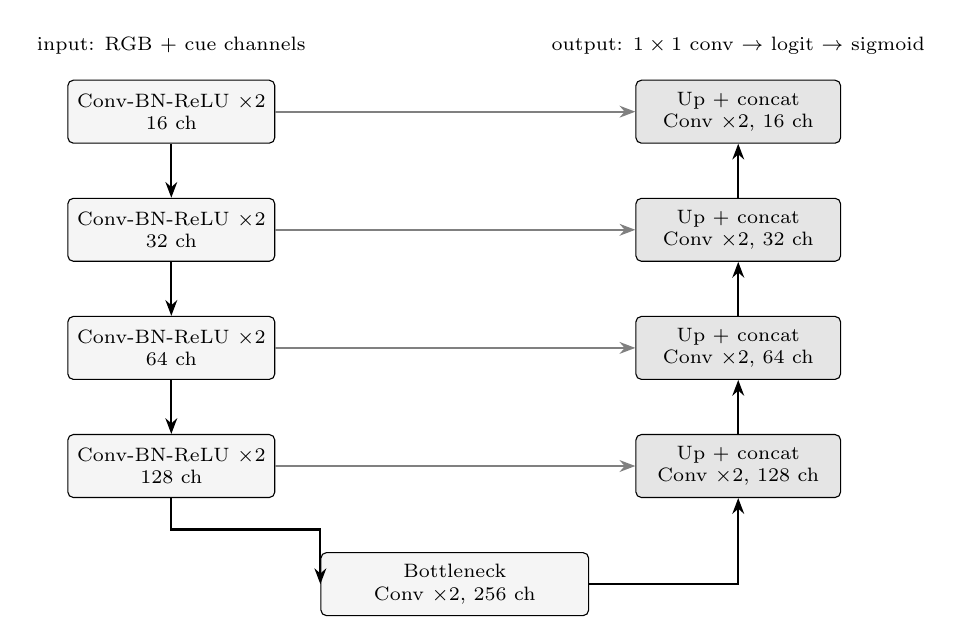
\begin{tikzpicture}[
  blk/.style={draw,rounded corners=2pt,align=center,font=\scriptsize,minimum width=2.6cm,minimum height=0.8cm,fill=gray!8},
  dec/.style={blk,fill=gray!20},
  arr/.style={-{Stealth[length=2mm]},thick},
  skip/.style={-{Stealth[length=2mm]},gray,thick}]
\node[blk] (e1) at (0,0) {Conv-BN-ReLU $\times2$\\16 ch};
\node[blk] (e2) at (0,-1.5) {Conv-BN-ReLU $\times2$\\32 ch};
\node[blk] (e3) at (0,-3.0) {Conv-BN-ReLU $\times2$\\64 ch};
\node[blk] (e4) at (0,-4.5) {Conv-BN-ReLU $\times2$\\128 ch};
\node[blk,minimum width=3.4cm] (bn) at (3.6,-6.0) {Bottleneck\\Conv $\times2$, 256 ch};
\node[dec] (d4) at (7.2,-4.5) {Up + concat\\Conv $\times2$, 128 ch};
\node[dec] (d3) at (7.2,-3.0) {Up + concat\\Conv $\times2$, 64 ch};
\node[dec] (d2) at (7.2,-1.5) {Up + concat\\Conv $\times2$, 32 ch};
\node[dec] (d1) at (7.2,0) {Up + concat\\Conv $\times2$, 16 ch};
\node[font=\scriptsize,above=2mm of e1] {input: RGB + cue channels};
\node[font=\scriptsize,above=2mm of d1] {output: $1\times1$ conv $\to$ logit $\to$ sigmoid};
\draw[arr] (e1)--(e2); \draw[arr] (e2)--(e3); \draw[arr] (e3)--(e4);
\draw[arr] (e4.south)--++(0,-0.4)-|(bn.west);
\draw[arr] (bn.east)-|(d4.south);
\draw[arr] (d4)--(d3); \draw[arr] (d3)--(d2); \draw[arr] (d2)--(d1);
\foreach \a/\b in {e1/d1,e2/d2,e3/d3,e4/d4} \draw[skip] (\a.east)--(\b.west);
\end{tikzpicture}}
\caption{Compact U-Net-style segmenter. Grey arrows are skip connections that concatenate encoder features into the decoder.}
\end{figure}

\begin{table}[H]
\centering
\caption{Proposed layer plan. Input height 288 divides evenly by 16, so four poolings introduce no padding.}
\footnotesize
\begin{tabular}{|l|l|l|}
\hline
\rowcolor{gray!18}\textbf{Stage}&\textbf{Size at $512\times288$}&\textbf{Channels}\\ \hline
Encoder 1 & $512\times288$ & 16\\ \hline
Encoder 2 & $256\times144$ & 32\\ \hline
Encoder 3 & $128\times72$ & 64\\ \hline
Encoder 4 & $64\times36$ & 128\\ \hline
Bottleneck & $32\times18$ & 256\\ \hline
Decoder 4 to 1 & Mirror of encoder & 128, 64, 32, 16\\ \hline
Output & $512\times288$ & 1 logit\\ \hline
\end{tabular}
\end{table}

For this layout the analytical parameter count is 1,944,049 for a 3-channel input and 1,944,337 for the 5-channel hybrid input (counting convolution weights and biases and batch-norm scale and shift). The two differ only in the first convolution, by 144 weights per extra input channel, so the ablation compares models of essentially equal capacity. These counts are arithmetic from the proposed plan and must be replaced by the count reported by the actual framework.

\subsection{Loss Function}
Binary cross-entropy with a positive-class weight $w$ penalizes a missed lane pixel $w$ times more than a false alarm:
\begin{equation}
\mathcal{L}_{\mathrm{BCE},w} = -\frac{1}{N}\sum_i\big[w\,y_i\log p_i+(1-y_i)\log(1-p_i)\big].
\end{equation}
A starting heuristic is $w=\min(w_{\max},N_{\mathrm{neg}}/N_{\mathrm{pos}})$ computed on training masks, with $w_{\max}$ capping the value because aggressive weighting raises false positives. The soft Dice term in Eq.~(\ref{eq:dice}) is computed on probabilities and is less affected by the background count. Focal loss \cite{lin2017} is an alternative that down-weights easy background pixels; it is listed as an optional comparison, not as part of the baseline.

\subsection{Optimization and Schedule}
Adam or AdamW with an initial learning rate of $10^{-3}$ is the proposed start. A reduce-on-plateau or cosine schedule may be tried; whichever is used is declared before the run and kept identical across ablations. Early stopping watches validation IoU with a predeclared patience, and the best-IoU checkpoint is the one frozen. Mixed-precision training may be enabled to fit memory, provided it is recorded in the configuration.

\subsection{Stability and Regularization}
Thin-structure segmentation can be unstable in early epochs because the positive class is rare. Practical safeguards include a short learning-rate warm-up, gradient-norm clipping, and weight decay when AdamW is used. Batch normalization depends on batch statistics, so very small batches, which may be forced by GPU memory, can degrade it; group normalization is a drop-in alternative that must be applied to every ablation if adopted. Whichever options are chosen are recorded in the configuration and held constant across A0 to A4.

\subsubsection*{Dataset Preparation and Training Pseudocode}
The outline makes the sequence-level split before model selection, keeps geometric transforms aligned with masks, and selects the checkpoint and probability threshold using validation data only. The held-out test split is evaluated after these choices are frozen.

\begin{lstlisting}
function train_lane_model(dataset, config):
  manifest = read_frames_and_lane_annotations(dataset)
  train_ids, val_ids, test_ids =
      split_by_video_sequence(manifest, config.seed)
  for sample in manifest:
    sample.mask = rasterize_lanes(
        sample.points, config.mask_width,
        config.ignore_policy)
    sample.cues = make_roi_color_edge_cues(
        sample.rgb, config.roi, config.canny)
  train = loader(train_ids, aligned_augmentation=True)
  valid = loader(val_ids, augmentation=False)
  model = initialize_unet(RGB_channels + cue_channels)
  optimizer = initialize_optimizer(model, config)
  best_iou = -infinity
  for epoch in 1..config.max_epochs:
    for rgb, mask, cues in train:
      x = normalize(concat(rgb, cues), train_stats)
      logits = model(x)
      loss = weighted_BCE(logits, mask)
      loss += config.lambda * soft_Dice_loss(logits, mask)
      optimizer.zero_grad()
      backpropagate(loss)
      optimizer.step()
    metrics = evaluate(model, valid, config.thresholds)
    if metrics.IoU > best_iou:
      save_model_optimizer_config(model, optimizer, config)
      best_iou = metrics.IoU
    if early_stopping(metrics, config.patience):
      break
  tau = select_threshold(best_checkpoint, valid)
  test = evaluate_frozen(best_checkpoint, test_ids, tau)
  save_metrics_config_and_logs(test, config, tau)
  return best_checkpoint, tau, test
\end{lstlisting}

\begin{table}[H]
\centering
\caption{Proposed experimental configuration; replace with actual values.}
\footnotesize
\begin{tabularx}{\columnwidth}{|l|X|}
\hline
\rowcolor{gray!18}\textbf{Parameter}&\textbf{Proposed setting}\\ \hline
Dataset & CULane official split; record version and counts\\ \hline
Input & $512\times288$ starting point\\ \hline
Model & U-Net-style binary segmenter; record channels and parameter count\\ \hline
Optimizer & Adam or AdamW; log exact parameters\\ \hline
Learning rate & $10^{-3}$ starting point; select on validation\\ \hline
Batch / epochs & Fill actual batch; maximum 50 with early stopping\\ \hline
Loss & Weighted BCE + soft Dice; record weights\\ \hline
Threshold & 0.50 initial; tune on validation only\\ \hline
Seeds & 42, 43, 44 if repeated runs are feasible\\ \hline
Hardware / software & Record device, memory, OS, and exact package versions\\ \hline
\end{tabularx}
\end{table}

Use the same sequence-level split, resolution, augmentation, optimizer, training budget, and network capacity for each ablation. Include a traditional-only Canny/geometry baseline when feasible. Run at least three seeds if resources permit; otherwise state that results are from one run. Moderate brightness/contrast, small translations/scales, and mild blur may improve coverage. Avoid physically implausible augmentation. Use early stopping with a predeclared patience. The software stack is PyTorch \cite{paszke2019} with OpenCV for the classical stage.

\subsection{Ablation Design}\label{sec:ablation}
\begin{table}[H]
\centering
\caption{Ablation matrix. A0 to A4 share split, resolution, optimizer, schedule, and training budget; only the input channels change.}
\footnotesize
\begin{tabular}{|l|l|c|}
\hline
\rowcolor{gray!18}\textbf{ID}&\textbf{Input channels}&\textbf{In-ch.}\\ \hline
B0 & Canny + geometry only (no network) & n/a\\ \hline
A0 & RGB (CNN-only baseline) & 3\\ \hline
A1 & RGB + ROI & 4\\ \hline
A2 & RGB + edge & 4\\ \hline
A3 & RGB + ROI + edge (hybrid) & 5\\ \hline
A4 & A3 + Hough support (optional) & 6\\ \hline
\end{tabular}
\end{table}

\subsection{Post-Processing and Its Separate Reporting}
After thresholding, the mask is restricted to the ROI and tiny connected components are removed. Optional curve fitting can summarize each lane as a polynomial in image coordinates. Because these steps can hide model errors, every metric is reported twice: once on the raw thresholded network output and once after post-processing. The difference between the two rows is the measured contribution of post-processing.

\section{Evaluation}\label{sec:eval}
Define TP as correctly predicted lane pixels, FP as background predicted as lane, FN as missed lane pixels, and TN as correctly predicted background. State whether metrics are global over pixels or macro-averaged per image; report both where practical. The principal overlap measures are
\begin{equation}
\mathrm{IoU}=\frac{TP}{TP+FP+FN},\qquad
\mathrm{Dice}=F_1=\frac{2\,TP}{2\,TP+FP+FN}.
\end{equation}
Also report pixel accuracy $(TP+TN)/(TP+TN+FP+FN)$, precision $TP/(TP+FP)$, and recall $TP/(TP+FN)$. Accuracy must not be used alone because background dominates. Document zero-denominator and ignored-pixel handling.

Measure preprocessing, network inference, and total latency separately after warm-up on a stated device and image size; report mean, median, and frames per second. Inspect overlays for shadows, curves, intersections, worn paint, night scenes, and occlusions. Runtime must be measured, not inferred from architecture.

Specify the evaluation unit and averaging policy. Global pixel scores pool TP, FP, FN, and TN across all frames, while macro per-image averages give each frame equal weight and prevent long or large frames from dominating. Report both where practical. State how ignored pixels are excluded and how zero denominators are handled. Evaluate the threshold selected on validation data without retuning it on test data. Keep raw network predictions and post-processed predictions separate so the contribution of ROI restriction, component removal, or curve fitting remains visible. Scenario-wise results should use the dataset's available condition tags and should include exact counts.

\subsection{Why Accuracy Misleads: An Arithmetic Illustration}
The following numbers are invented only to show arithmetic; they are not measurements of this system. Take one $512\times288$ frame (147,456 pixels) with $TP=1{,}400$, $FP=700$, and $FN=800$, so $TN=144{,}556$. Then accuracy is 0.9898, yet IoU is 0.483, Dice is 0.651, precision is 0.667, and recall is 0.636. A trivial model that predicts only background on the same frame reaches accuracy 0.9851 with an IoU of zero. High accuracy therefore says almost nothing about lane quality here.

\subsection{Zero Denominators and Ignored Pixels}
A frame with no lane pixels in either prediction or label has $TP+FP+FN=0$, making IoU undefined. The protocol fixes one rule in advance, for example scoring such a frame as 1 when the prediction is also empty and 0 otherwise, and applies it to every model. Pixels marked ignored in the label are removed from all four counts before any metric is computed.

\subsection{Latency Protocol}
Latency is split as $t_{\mathrm{total}}=t_{\mathrm{pre}}+t_{\mathrm{net}}+t_{\mathrm{post}}$, and throughput is the reciprocal of the mean total time. Run a warm-up of several frames before timing; on a GPU, synchronize the device before reading the clock so that asynchronous kernels are not undercounted. Report mean and median, the device, the input size, and whether decoding and display are inside or outside the timed region.

\subsection{Variability and Comparison}\label{sec:variability}
With three or more seeds, report the mean and standard deviation of each metric. A difference between two input configurations is treated as meaningful only if it is larger than the seed-to-seed spread and appears in several scenario categories. Frames from one sequence are correlated, so any resampling-based confidence interval should resample sequences, not individual frames.

\subsection{Scenario-Wise Reporting Template}
\begin{table}[H]
\centering
\caption{Template for per-category comparison; values must come from held-out evaluation.}
\footnotesize
\begin{tabular}{|l|l|l|l|l|}
\hline
\rowcolor{gray!18}\textbf{Category}&\textbf{Frames}&\textbf{IoU A0}&\textbf{IoU A3}&\textbf{Diff.}\\ \hline
Normal & count & FILL & FILL & FILL\\ \hline
Shadow & count & FILL & FILL & FILL\\ \hline
Night & count & FILL & FILL & FILL\\ \hline
Curve & count & FILL & FILL & FILL\\ \hline
Crossroad & count & FILL & FILL & FILL\\ \hline
\end{tabular}
\end{table}

\subsection{Qualitative Sampling}
Qualitative figures must not be cherry-picked. The protocol draws a fixed list of frame IDs per category using a recorded random seed before any model is evaluated, and every model is shown on the same IDs. In addition, the worst few frames by IoU in each category are shown, so that readers see failures as well as successes.

\section{Results}\label{sec:results}
No training run, dataset manifest, hardware log, or prediction output was supplied. Accordingly, this report presents no empirical performance figures. Results should be added only after evaluating predictions against held-out ground-truth masks with the protocol above.

Expected findings are hypotheses only: ROI and edge cues may improve localization where boundaries have strong gradients and reduce responses outside the road. Learned RGB context may recover faint or discontinuous paint missed by strict Canny thresholds. Noisy edges, fixed ROI geometry, and Hough assumptions may hurt at intersections, in shadows, at night, or on curves. Held-out IoU and latency determine whether hybrid inputs help.

\begin{table}[H]
\centering
\caption{Hypotheses and the evidence that would support each. None is yet tested.}
\footnotesize
\begin{tabularx}{\columnwidth}{|l|X|X|}
\hline
\rowcolor{gray!18}\textbf{ID}&\textbf{Hypothesis}&\textbf{Supported only if}\\ \hline
H1 & ROI channel lowers false positives outside the road & A1 precision above A0 across seeds\\ \hline
H2 & Edge channel helps faint paint & A2 recall above A0 in No-line and Night\\ \hline
H3 & Hybrid input improves IoU & A3 IoU above A0 by more than seed spread\\ \hline
H4 & Gains hold beyond easy scenes & Gain visible in Shadow and Curve too\\ \hline
H5 & Cues add little latency & $t_{\mathrm{pre}}$ small relative to $t_{\mathrm{net}}$\\ \hline
\end{tabularx}
\end{table}

\begin{table}[H]
\centering
\caption{Results template for held-out test data (mean $\pm$ std over seeds). Intentionally empty: no run was supplied.}
\footnotesize
\begin{tabular}{|l|c|c|c|c|c|}
\hline
\rowcolor{gray!18}\textbf{ID}&\textbf{IoU}&\textbf{Dice}&\textbf{Prec.}&\textbf{Rec.}&\textbf{ms/frame}\\ \hline
B0 & \multicolumn{5}{c|}{not measured}\\ \hline
A0 & \multicolumn{5}{c|}{not measured}\\ \hline
A1 & \multicolumn{5}{c|}{not measured}\\ \hline
A2 & \multicolumn{5}{c|}{not measured}\\ \hline
A3 & \multicolumn{5}{c|}{not measured}\\ \hline
\end{tabular}
\end{table}

\subsection*{Dashboard Demonstration}
Figures~\ref{fig:dash1} and~\ref{fig:dash2} document the LaneSight interface before and during processing. The displayed telemetry has not been independently benchmark-validated; these screenshots document the prototype interface and are not evidence of measured model performance.

\begin{figure}[H]
\centering
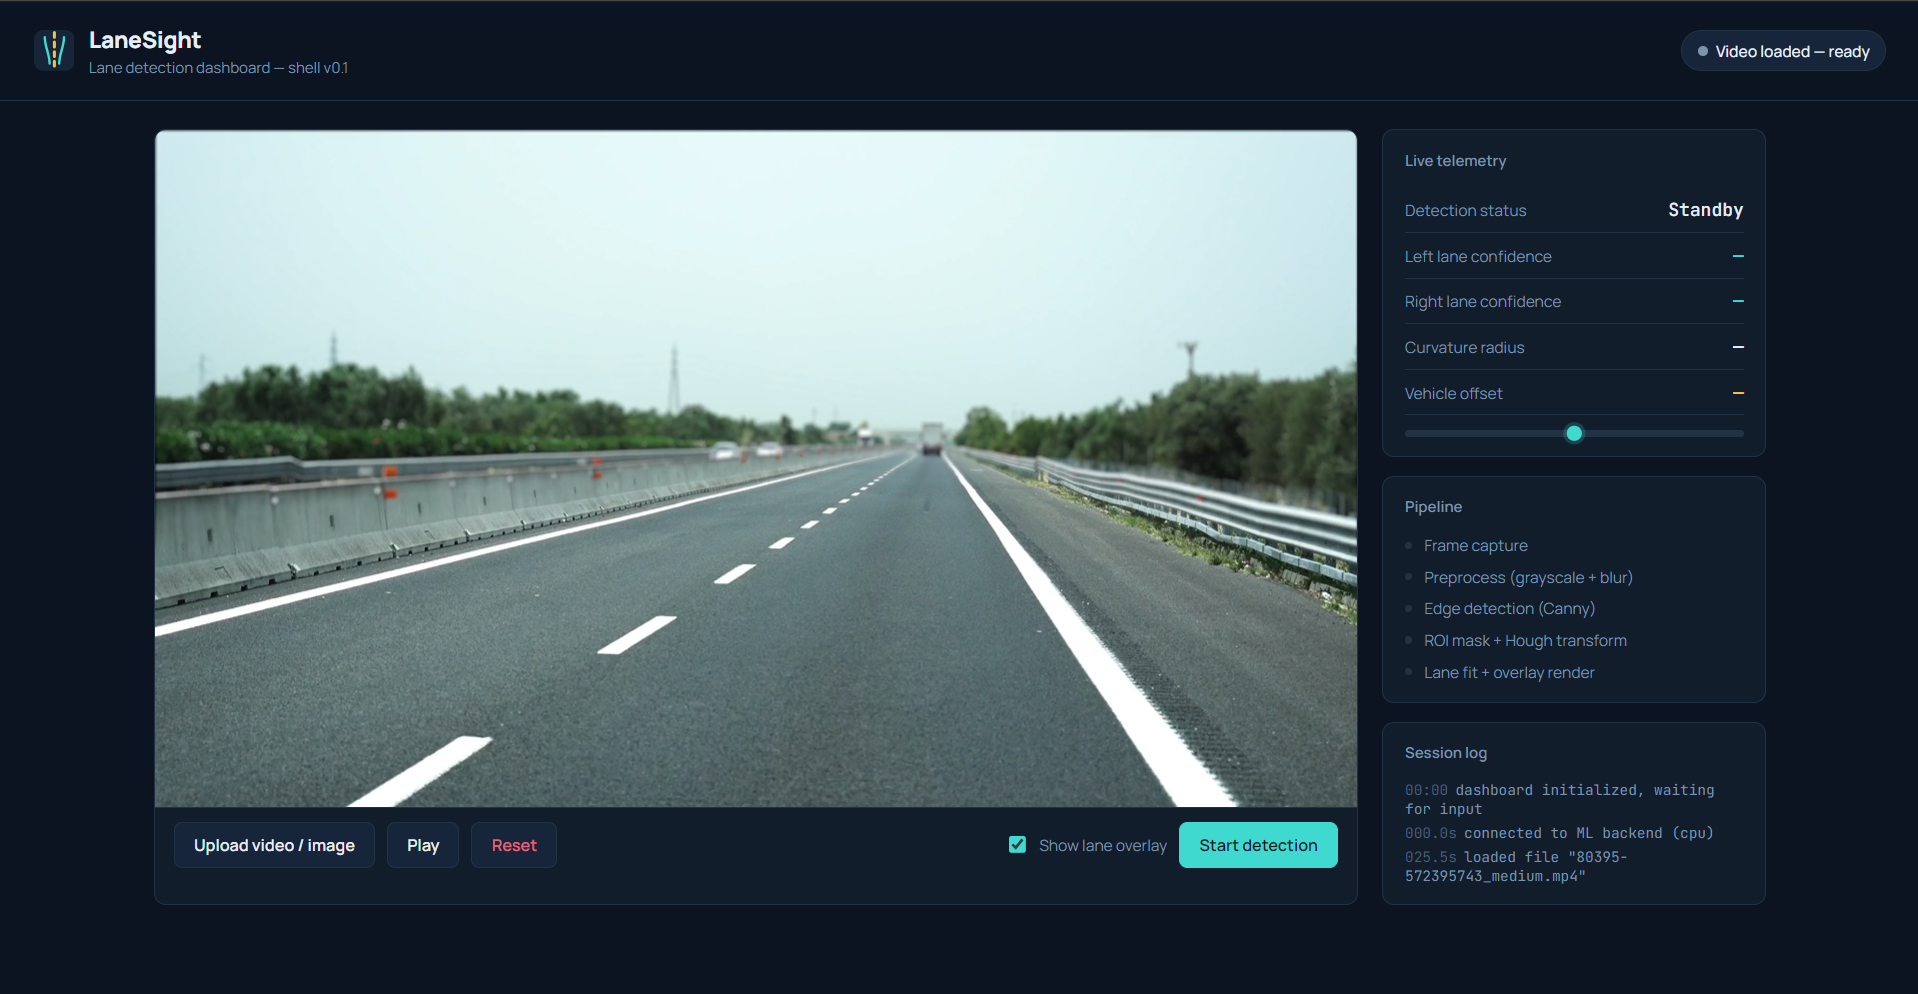
\includegraphics[width=\columnwidth]{lane_detection_dashboard_ready.png}
\caption{LaneSight dashboard with a road video loaded before detection begins.}\label{fig:dash1}
\end{figure}

\begin{figure}[H]
\centering
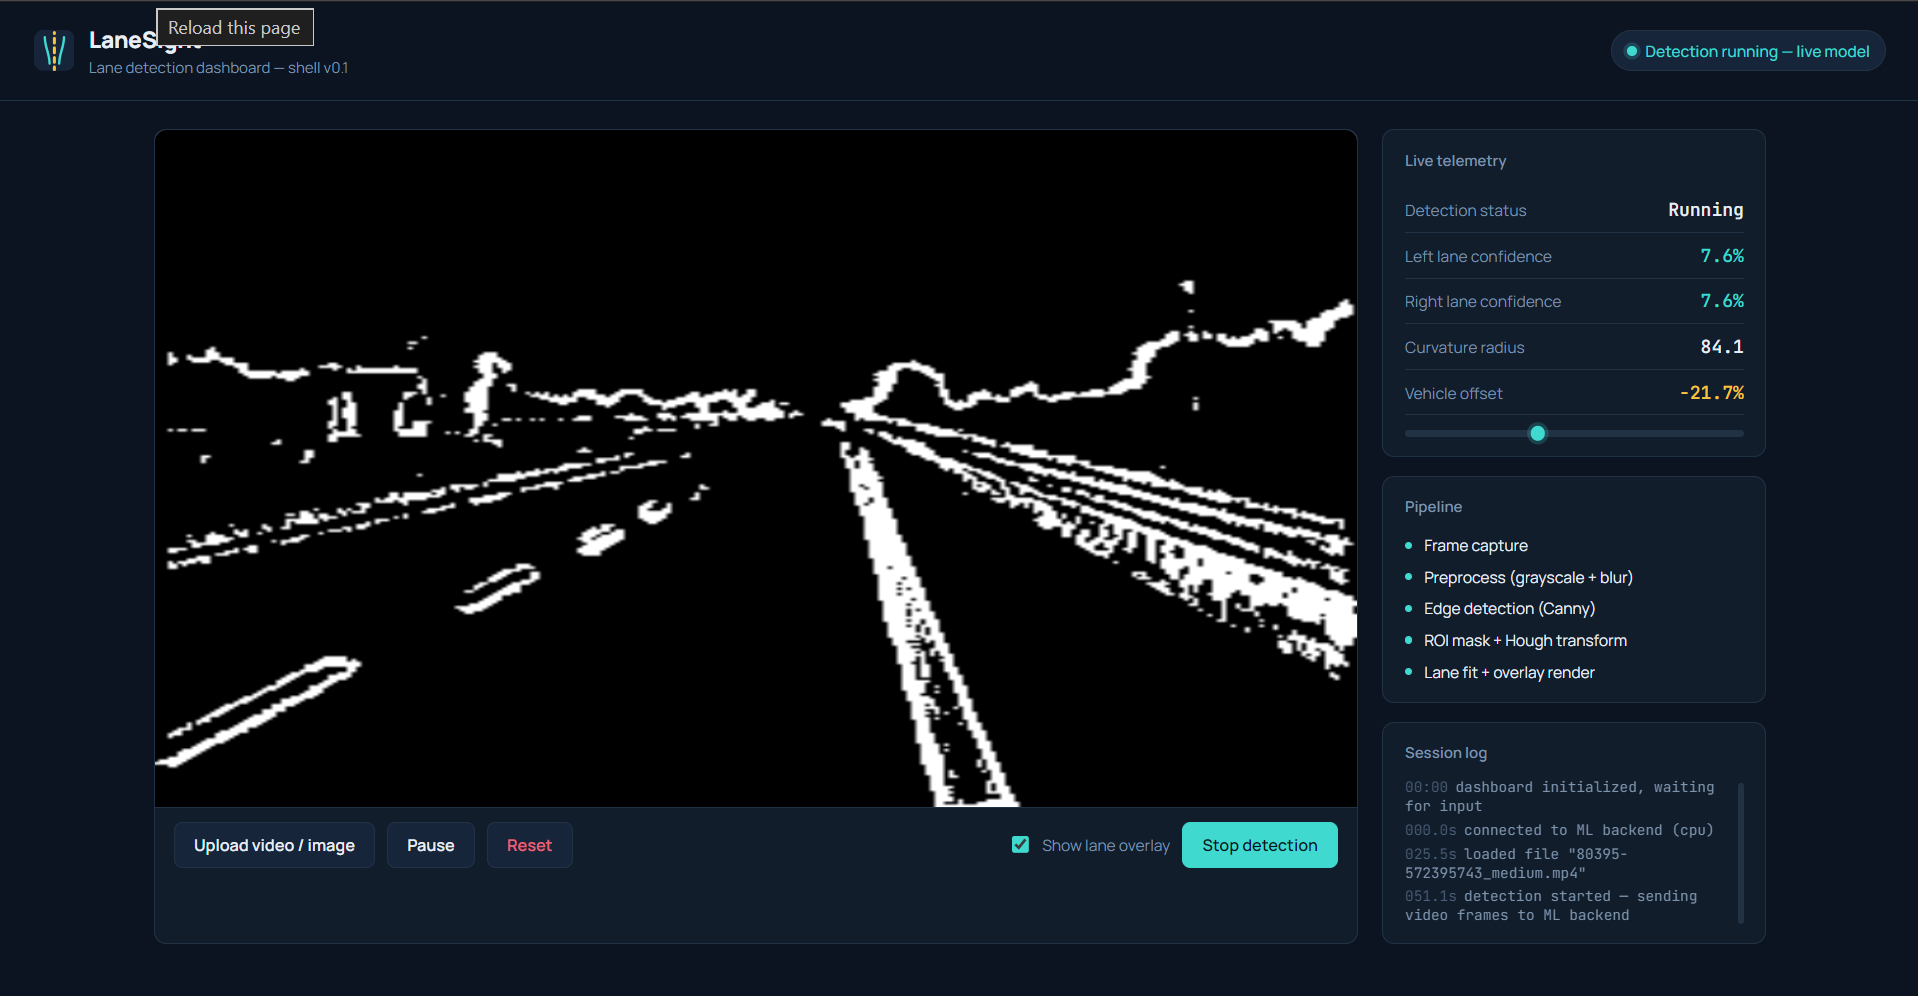
\includegraphics[width=\columnwidth]{lane_detection_dashboard_running.png}
\caption{LaneSight processing view and displayed telemetry; values are not benchmark-validated.}\label{fig:dash2}
\end{figure}

\subsection{Reading the Dashboard}
The interface has a video panel with upload, play, reset, and overlay controls; a live telemetry panel with detection status, left and right lane confidence, curvature radius, and vehicle offset; a pipeline checklist that lists frame capture, grayscale and blur preprocessing, Canny edge detection, ROI masking with Hough transform, and lane fit with overlay rendering; and a session log. In the processing view the video panel shows a white-on-black binary map, which corresponds to the classical edge stage. The telemetry numbers visible in that view, such as the confidence percentages, curvature value, and vehicle offset, are interface outputs only. They were not computed against labeled data, so they must not be quoted as accuracy or as lane-offset measurements.

\subsection{Wording Guide for Reporting}
Claims in the final report should match the evidence available at the time of writing. The table contrasts wording that overstates the evidence with wording that stays within it.

\begin{table}[H]
\centering
\caption{Overstated versus evidence-bound wording.}
\footnotesize
\begin{tabularx}{\columnwidth}{|X|X|}
\hline
\rowcolor{gray!18}\textbf{Avoid}&\textbf{Use instead}\\ \hline
The system detects lanes accurately & On held-out CULane frames the model reached IoU = FILL (mean, $n$ seeds)\\ \hline
Works in real time & Mean total latency was FILL ms on DEVICE at $512\times288$\\ \hline
Edge cues improve results & A3 exceeded A0 by FILL IoU, larger / not larger than seed spread\\ \hline
Robust to all conditions & Scores in Night and Shadow were FILL and FILL\\ \hline
Safe for driver assistance & The prototype is academic and not safety validated\\ \hline
\end{tabularx}
\end{table}

\section{Discussion}\label{sec:discussion}
ROI masking and conventional filtering make preprocessing inspectable and may limit irrelevant candidates. Pixel-wise learning adds semantic context that thresholding and straight-line fitting lack. The key question is whether extra cues improve a CNN-only model consistently rather than only producing appealing overlays on selected examples.

Interpret overlap together with error type. Higher precision but lower recall suggests a conservative model that misses faint paint; higher recall but lower precision may reflect false responses on seams, curbs, or vehicle edges. Per-condition scores and overlays help locate failures in ROI choice, cue generation, mask rasterization, or classification. Compare CNN-only, CNN+ROI, CNN+edge, and full hybrid inputs across seeds and scenario groups. Control or disclose differences in compute, parameters, resolution, and training budget.

A gain that persists across seeds and difficult scenario groups would support the value of traditional cues. A gain limited to simple daytime scenes would suggest weaker generalization. High pixel accuracy can coexist with poor IoU because background dominates. Therefore, show representative correct detections and failure cases rather than selecting only favorable frames. Discuss whether false responses concentrate at road seams, curbs, shadows, or vehicle edges, and whether missed markings are faint, occluded, or outside the fixed ROI. The dashboard's displayed confidence or latency should not be described as a benchmark result unless it is independently measured against a stated protocol.

\subsection{Error Taxonomy}
\begin{table}[H]
\centering
\caption{Error types, probable causes, and the diagnostic used to confirm each.}
\footnotesize
\begin{tabularx}{\columnwidth}{|X|X|X|}
\hline
\rowcolor{gray!18}\textbf{Error}&\textbf{Likely cause}&\textbf{Diagnostic}\\ \hline
Thick or doubled lane & Mask width, resize blur & Overlay at native size\\ \hline
Missed dashed paint & Strict Canny, closing too small & Edge map vs.\ mask\\ \hline
Response on seam or curb & Strong gradient, weak context & Per-category precision\\ \hline
Mask outside road & ROI too wide or absent & Raw vs.\ ROI-masked\\ \hline
Lane cut off on bend & Fixed ROI too narrow & Curve category recall\\ \hline
Flicker between frames & Single-frame inference & Frame-to-frame IoU\\ \hline
\end{tabularx}
\end{table}

\subsection{Threats to Validity}
Internal validity is threatened by tuning on test data, by unequal training budgets across ablations, and by seed luck; the protocol addresses these through a frozen test split, a shared budget, and repeated seeds. External validity is threatened by camera and country differences: a model trained on CULane may not transfer to Indian roads without separate evaluation. Construct validity is threatened by metric choice: pixel IoU on thin lines is harsh for small localization offsets, so a tolerance-based measure may be added as a secondary view while the pixel metrics remain primary.

\subsection{Role of the Traditional-Only Baseline}
The traditional-only baseline B0 is not expected to match a trained network on hard scenes, and it is not included to be beaten cheaply. Its purpose is to show what the classical stage contributes on its own, to give a latency floor, and to make explicit which scenes are solvable without learning. If B0 is competitive on normal highway frames but collapses on shadow and night frames, that pattern supports using it as a source of cues rather than as the decision maker.

\section{Limitations}\label{sec:limits}
Performance depends on dataset coverage and annotation consistency; rasterization width can make boundaries too thick or thin. A single camera predicts image pixels, not true road geometry. ROI vertices, Canny thresholds, morphology kernels, and Hough parameters depend on camera mounting, resolution, and scene composition. Pixel labels are imbalanced, and aggressive weighting can increase false positives. A benchmark-trained model may not generalize across countries, optics, marking conventions, weather, or night exposure. Single-frame processing may flicker; temporal tracking is outside scope. Without training and test execution, no accuracy, robustness, or real-time claim is supported. The prototype is not safety validated.

Additional limitations follow from the design choices. A fixed rasterization width can encode an arbitrary boundary thickness, while poorly aligned image and mask transforms can corrupt labels. The ROI can exclude valid lanes on crests or sharp curves. Hough assumptions work best for approximately straight segments and may fail under occlusion or strong curvature. The learned model requires labeled data and compute, and its outputs may shift with camera optics or road-marking conventions. These risks should be reported alongside any future measured metrics; a single-frame academic prototype must not be presented as a production driver-assistance component.

\begin{table}[H]
\centering
\caption{Project risk register.}
\footnotesize
\begin{tabularx}{\columnwidth}{|X|X|X|}
\hline
\rowcolor{gray!18}\textbf{Risk}&\textbf{Effect}&\textbf{Mitigation}\\ \hline
Label leakage across frames & Inflated scores & Sequence-level split\\ \hline
Mask / image misalignment & Corrupted labels & Joint transforms; overlay check\\ \hline
Threshold tuned on test & Optimistic result & Freeze before test\\ \hline
Limited GPU memory & Smaller batch or size & Report values; keep equal across runs\\ \hline
Single seed only & Unknown variance & State limitation directly\\ \hline
Dataset license limits & Cannot share frames & Share manifests and code only\\ \hline
\end{tabularx}
\end{table}

\section{Reproducibility and Future Work}\label{sec:repro}
Store code, configuration, data manifest, seeds, package versions, checkpoint rule, and evaluation script version. Keep test data read-only during model selection. Export masks and overlays for fixed sample IDs. Suggested artifacts include a dataset manifest, preprocessing configuration, training log, checkpoint, test and condition metrics, predictions, and README. Do not redistribute dataset frames unless permitted.

Future work can add temporal tracking with frame-level failure reporting; multi-class lane instances where labels are reliable; lightweight backbones, quantization, and hardware acceleration; safe local Indian-road evaluation; camera calibration and bird's-eye transforms; cross-dataset testing; and uncertainty estimates that allow low-confidence abstention.

The software stack should be stated precisely in the final project report. OpenCV can implement image processing; PyTorch can implement the segmenter and training loop; NumPy and Pillow/OpenCV can support data handling and overlays; Matplotlib or OpenCV can render diagnostics. Log color order, ROI vertices, Canny thresholds, morphology kernel shape and size, mask-width rule, loss weights, optimizer settings, seed, epoch count, and metric averaging policy. Preserve a model state dictionary, machine-readable configuration, package versions, hardware details, training log, split manifest, test metrics, condition metrics, and fixed-ID prediction overlays. A webcam or video interface is optional and should display confidence and measured processing latency without implying safety validation.

Further extensions include testing multi-class left/right or lane-instance identities only when annotations are reliable; measuring temporal stability without hiding frame-level failures; evaluating lightweight backbones, pruning, quantization, and hardware acceleration for embedded devices; and testing on locally collected Indian-road scenes acquired safely and with appropriate privacy practices. Camera calibration and bird's-eye transforms could support road-width or curvature estimates, which remain outside the current image-mask objective. Cross-dataset evaluation and domain adaptation should use data not involved in tuning. Uncertainty estimation can provide a low-confidence state for abstention.

\subsection{Proposed Work Plan}
\begin{table}[H]
\centering
\caption{Phases in dependency order; durations depend on available compute.}
\footnotesize
\begin{tabularx}{\columnwidth}{|l|X|l|}
\hline
\rowcolor{gray!18}\textbf{Phase}&\textbf{Work}&\textbf{Output}\\ \hline
1 & Obtain data; build manifest and split & Manifest file\\ \hline
2 & Implement and inspect classical cues & Intermediate images\\ \hline
3 & Rasterize masks; check overlays & Mask set\\ \hline
4 & Train A0 baseline & Checkpoint, log\\ \hline
5 & Train A1 to A3 under equal budget & Ablation logs\\ \hline
6 & Select threshold on validation; freeze & Frozen config\\ \hline
7 & Evaluate on test; latency; scenarios & Metrics files\\ \hline
8 & Write results; failure cases & Final report\\ \hline
\end{tabularx}
\end{table}

\subsection{Suggested Repository Layout}
\begin{lstlisting}
lane-hybrid/
  configs/    base.yaml, ablation_*.yaml
  data/       manifests/ (frames not redistributed)
  src/
    cues.py       roi, canny, morphology, hough
    dataset.py    loader, rasterize, augmentation
    model.py      U-Net-style segmenter
    train.py      loop, checkpoint, early stopping
    evaluate.py   metrics, latency, per-scenario
    infer.py      video -> overlays + log
  runs/<id>/  config, log, checkpoint, metrics
  README.md
\end{lstlisting}

\subsection{Ethics and Privacy}
Driving video can contain faces and license plates. Locally collected footage should be captured safely and without handling a camera while driving, and published frames should be blurred or omitted where individuals can be identified. Benchmark data must be used under their own terms.

\subsection{Toward Embedded Deployment}
A natural continuation is running the trained segmenter on an embedded board. Candidate steps are exporting the model to an interchange format, post-training quantization to 8-bit integers, reducing input resolution, and moving the classical stage to optimized library calls. Each step can change both accuracy and latency, so each must be re-evaluated with the same protocol and reported next to the original floating-point result. No embedded performance is claimed in this report.

\subsection{Code Availability}
The source code and the LaneSight dashboard prototype for this project are available in the authors' GitHub repositories \url{https://github.com/Sujal-48/Lane-Detection-System} and \url{https://github.com/nitishgupta2764-cmd/Lane-Detection-System}.

\section{Conclusion}
This report specifies a hybrid lane-detection system for an ECE project. Traditional vision supplies road-region selection and edge/color/geometric cues through ROI masking, color and grayscale conversion, Gaussian blur, Canny detection, morphology, and optional Hough or curve fitting. A U-Net-style model performs the central pixel-wise classification. The report defines data preparation, training, validation, ablations, evaluation, and reproducibility. Because no project-specific training or test outputs were supplied, no performance figures are reported. The CNN-only comparison and held-out evaluation provide a path from this design specification to an empirical project report.

\section*{Acknowledgments and Disclosure of Funding}
The dataset creators and authors of cited methods are acknowledged for making benchmark resources and research available. No external funding or project-specific experimental contribution is asserted.

\appendix
\titleformat{\section}{\large\bfseries}{Appendix \thesection:}{0.5em}{}

\section{End-to-End Pipeline and Reporting Checklist}
\textbf{Training:} manifest and lane-polyline rasterization; aligned resize and augmentation; training-only normalization; optimization; validation checkpoint and threshold selection; frozen test evaluation; saved metrics and overlays. \textbf{Inference:} road frame; color/grayscale conversion; smoothing; ROI and Canny cues; morphology or optional Hough; tensor assembly; U-Net probabilities; validation-selected threshold; optional refinement; overlay and metrics.

Before reporting results, record split counts, mask width, ignore policy, interpolation, ROI coordinates, seed count, model size, hardware, software, training time, macro and global metrics, all ablations, condition-level results, and latency. Show representative successes and failures, and label results as measured only after held-out evaluation. Suggested project outputs are a dataset manifest, preprocessing configuration, training log, best checkpoint, test-metrics file, condition-metrics file, prediction masks, overlays, and a README. Do not include redistributed dataset frames unless the applicable dataset terms allow it. These are reproducibility recommendations; no such run files or model artifacts were included with the report.

\section{Configuration Template}
\begin{lstlisting}
seed: [42, 43, 44]
data: {name: CULane, release: FILL, split: FILL}
input: {size: [512, 288], color_order: RGB}
roi: {vertices: FILL, normalized: true}
canny: {low: FILL, high: FILL, blur: 5}
morph: {op: close, kernel: [3, 3]}
mask: {width: FILL, ignore_gap: FILL}
model: {channels: [16,32,64,128,256], in_ch: 5}
loss: {pos_weight: FILL, lambda_dice: 0.5}
optim: {name: AdamW, lr: 1.0e-3, batch: FILL}
train: {max_epochs: 50, patience: FILL}
eval: {threshold: select_on_val, avg: [global, macro]}
\end{lstlisting}

\section{Notation}
\begin{table}[H]
\centering
\caption{Symbols used in this report.}
\footnotesize
\begin{tabular}{|l|l|}
\hline
\rowcolor{gray!18}\textbf{Symbol}&\textbf{Meaning}\\ \hline
$I, H, W$ & Image, height, width\\ \hline
$R$ & Binary ROI mask\\ \hline
$C(\cdot)$ & Deterministic classical cue generator\\ \hline
$f_\theta$ & Segmentation network with parameters $\theta$\\ \hline
$p_i, y_i$ & Predicted probability and target of pixel $i$\\ \hline
$\tau$ & Validation-selected probability threshold\\ \hline
$w, \lambda, \varepsilon$ & Positive-class weight, Dice weight, smoothing\\ \hline
\end{tabular}
\end{table}

\section{Glossary}
\begin{table}[H]
\centering
\caption{Glossary of terms.}
\footnotesize
\begin{tabularx}{\columnwidth}{|l|X|}
\hline
\rowcolor{gray!18}\textbf{Term}&\textbf{Meaning}\\ \hline
ROI & Region of interest: the image area where lanes are expected\\ \hline
Hysteresis & Two-threshold rule that keeps weak edges linked to strong ones\\ \hline
Skip connection & Link that passes encoder features to the decoder\\ \hline
Dice / F1 & Overlap score $2TP/(2TP+FP+FN)$\\ \hline
IoU & Intersection over union of predicted and true lane pixels\\ \hline
Ablation & Experiment that changes one component at a time\\ \hline
Domain shift & Change between training and deployment data\\ \hline
Macro / global & Per-image average vs.\ pooled pixel counts\\ \hline
\end{tabularx}
\end{table}

\section{Final Submission Checklist}
\begin{table}[H]
\centering
\caption{Checklist to complete before the results are written.}
\footnotesize
\begin{tabular}{|l|l|}
\hline
\rowcolor{gray!18}\textbf{Item}&\textbf{Status}\\ \hline
Manifest, split counts, license note recorded & To do\\ \hline
Overlays inspected for every category & To do\\ \hline
All ablations trained under equal budget & To do\\ \hline
Threshold and ROI frozen before test & To do\\ \hline
Raw and post-processed metrics reported & To do\\ \hline
Latency measured with warm-up & To do\\ \hline
Success and failure figures included & To do\\ \hline
Limitations and non-safety statement kept & To do\\ \hline
\end{tabular}
\end{table}

\section{Metric Computation Reference}
The routine below computes the overlap metrics from a predicted mask, a label mask, and an ignore mask. It is written so that the zero-denominator rule of Section~\ref{sec:eval} is explicit and identical for every model.

\begin{lstlisting}[caption={Metric computation with explicit empty-frame handling.}]
function metrics(pred, label, ignore, empty_score=1.0):
  valid = NOT ignore
  TP = sum((pred AND label) AND valid)
  FP = sum((pred AND NOT label) AND valid)
  FN = sum((NOT pred AND label) AND valid)
  TN = sum((NOT pred AND NOT label) AND valid)
  if TP + FP + FN == 0:
    iou = empty_score       # both empty: fixed rule
    dice = empty_score
  else:
    iou = TP / (TP + FP + FN)
    dice = 2*TP / (2*TP + FP + FN)
  prec = TP / (TP + FP) if TP + FP > 0 else None
  rec  = TP / (TP + FN) if TP + FN > 0 else None
  acc = (TP + TN) / (TP + TN + FP + FN)
  return TP, FP, FN, TN, iou, dice, prec, rec, acc

function aggregate(frames):
  glob = metrics_from_sums(sum_counts(frames))   # pooled
  macro = mean(f.iou for f in frames)            # per image
  return glob, macro
\end{lstlisting}

\section{Determinism and Seeding Notes}
Exact bit-for-bit repeatability on a GPU is not always possible, because some kernels are non-deterministic. The aim here is the weaker, honest goal of controlled variability: set the seeds of the random number generators used by the framework, by NumPy, and by the data loader workers; enable deterministic algorithm settings where the framework offers them and note any operation that cannot be made deterministic; and record the framework and driver versions. When two runs with the same seed differ slightly, the difference is reported as a floor on run-to-run noise, and the seed-to-seed spread of Section~\ref{sec:variability} is interpreted against it.

The classical stage, in contrast, is fully deterministic on a given library version. Its output should therefore be identical between training and inference; the cue hash in the log record turns this expectation into a check. A mismatch indicates a different library version, color order, or configuration, and should be resolved before any metric is trusted.

\section{Run Record Template}
\begin{table}[H]
\centering
\caption{One record per run, stored with the checkpoint.}
\footnotesize
\begin{tabularx}{\columnwidth}{|l|X|}
\hline
\rowcolor{gray!18}\textbf{Field}&\textbf{Value to record}\\ \hline
Run ID, date & Unique label and start date\\ \hline
Ablation ID & B0, A0 to A4\\ \hline
Seed & 42, 43, or 44\\ \hline
Epochs run, best epoch & Integers from the log\\ \hline
Best validation IoU & From the checkpoint rule\\ \hline
Threshold selected & Value and selection rule\\ \hline
Training time, device & Wall clock and hardware\\ \hline
Parameter count & From the framework\\ \hline
\end{tabularx}
\end{table}

\section{Design Questions}
\textbf{Why not rely on Hough lines alone?} Straight-line votes fail on curves and under occlusion, and they cannot use context to reject seams or shadows. They remain useful as an optional cue and as a transparent baseline.

\smallskip\noindent\textbf{Why binary segmentation instead of lane instances?} A binary mask needs only one class, matches the available annotation rasterization, and keeps the first comparison simple. Instance identities can be added later where labels are reliable.

\smallskip\noindent\textbf{Why $512\times288$?} The height divides evenly by 16 for four poolings, the aspect ratio is close to the source video, and the size is small enough for a single modest GPU. It is a starting point to be reported, not an optimum.

\smallskip\noindent\textbf{Why recompute cues after augmentation?} It guarantees that the edge channel always describes the image the network actually sees, which removes a subtle source of train-time mismatch.

\begin{thebibliography}{99}\footnotesize
\bibitem{canny1986} J.~Canny, A computational approach to edge detection, \emph{IEEE Transactions on Pattern Analysis and Machine Intelligence} 8(6) (1986) 679--698. doi:10.1109/TPAMI.1986.4767851.
\bibitem{buslaev2020} A.~Buslaev et al., Albumentations: Fast and flexible image augmentations, \emph{Information} 11(2) (2020) 125. doi:10.3390/info11020125.
\bibitem{lin2017} T.-Y.~Lin et al., Focal loss for dense object detection, in: \emph{ICCV} (2017) 2980--2988. doi:10.1109/ICCV.2017.324.
\bibitem{neven2018a} D.~Neven, B.~De Brabandere, S.~Georgoulis, M.~Proesmans, and L.~Van Gool, LaneNet: Real-time lane detection networks for autonomous driving, arXiv:1807.01726 (2018).
\bibitem{neven2018b} D.~Neven et al., Towards end-to-end lane detection: An instance segmentation approach, arXiv:1802.05591 (2018).
\bibitem{pan2018} X.~Pan et al., Spatial as deep: Spatial CNN for traffic scene understanding, in: \emph{AAAI}, vol.~32 (2018). CULane project: \url{https://xingangpan.github.io/projects/CULane.html}.
\bibitem{paszke2019} A.~Paszke et al., PyTorch: An imperative style, high-performance deep learning library, in: \emph{NeurIPS}, vol.~32 (2019).
\bibitem{ronneberger2015} O.~Ronneberger, P.~Fischer, and T.~Brox, U-Net: Convolutional networks for biomedical image segmentation, in: \emph{MICCAI} (2015) 234--241. doi:10.1007/978-3-319-24574-4\_28.
\bibitem{tusimple} TuSimple, TuSimple benchmark: Lane detection challenge, dataset documentation and evaluation guideline, \url{https://github.com/TuSimple/tusimple-benchmark/tree/master/doc/lane_detection}.
\bibitem{yu2018} F.~Yu et al., BDD100K: A diverse driving dataset for heterogeneous multitask learning, arXiv:1805.04687 (2018).
\bibitem{authors2026} Sujal and N.~Gupta, Lane-Detection-System,
\\GitHub repositories (2026): \url{https://github.com/Sujal-48/Lane-Detection-System}; \url{https://github.com/nitishgupta2764-cmd/Lane-Detection-System}.
\end{thebibliography}

\end{document}